\subsection{Descripción general}
Los diagramas de actividad presentan varias caracteristicas que resultan ventajosas a la hora de especificar el comportamiento del sistema a desarrollar.
Principalmente la capacidad de los diagramas de actividad de especificar una secuencia de eventos resulta util para describir los procesos que ocurren en el ciclo de vida de los proyectos. Otra caracteristica relevante de esta herramienta es su capacidad de poder especificar procesos que suceden simultaneamente, es decir de forma paralela.

En particular, hemos confeccionado cuatro diagramas de actividad los cuales captan el ciclo de vida de los proyectos y las situaciones extraordinarias que suceden en la etapa de seguimiento, utilizando escenarios concretos. Detalladamente:

\begin{itemize}
  \item El primer diagrama de actividad confeccionado especifica un escenario completo del ciclo de vida de un proyecto con la particularidad de que suponemos que tanto el cliente como los proveedores utilizan el sistema, que, tanto el alcance como el presupuesto, son aceptados en el primer intento y que no hay inconvenientes en la etapa de seguimiento de los proyectos, es decir: el proveedor no cancela, el PM no es reemplazado y no cancela, y el PM carga las actualizaciones periodicas. Aclaramos que en este escenario el PM pide presupuestos a solo dos proveedores (llamados proveedor 1 y 2). Tomamos esta decisión porque el comportamiento del sistema no difiere si los pedidos de presupuesto son a 2 o a $N$ proveedores, mientras que con 2 proveedores ganamos claridad. Con respecto al resto de las caracteristicas particulares de este escenario, consideramos que para lograr captar al maximo el comportamiento del sistema y a su vez lograr que el diagrama sea legible, asumir que el cliente y el proveedor utilizan siempre el sistema es logico, lo mismo sucede con la definición del alcance y de presupuesto (proceso que se encuentra especificado en su totalidad en otra herramienta). Con respecto al seguimiento, consideramos que especificar todas las situaciones posibles en esta etapa en un diagrama resulta imposible por lo cual especificamos la situación ideal. El resto de los situaciones serán especificados en otros diagramas.

  \item El segundo diagrama de actividad especifica un escenario en donde el proveedor contratado (llamado proveedor 1 en el driagrama) cancela y se debe resolver esta situación extraordinaria. El mismo finaliza cuando un nuevo proveedor es contratado para llevar adelante la obra. Nuevamente limitamos la cantidad de proveedores a los que el sistema les pide presupuesto por las razones expuestas en el primer inciso. Este escenario representa una de las situaciones no especificadas en el primer diagrama, y, dado su importancia, consideramos necesario mostrarlo con un diagrama propio.

  \item El tercer diagrama de actividad especifica un escenario en donde el PM asignado es reemplazado debido a la inconformidad del cliente con respecto a su trabajo. El mismo finaliza con el reemplazo del PM por otro. Este escenario representa una de las situaciones no especificadas en el primer diagrama, y, dado su importancia, consideramos necesario mostrarlo con un diagrama propio.

  \item Por ultimo el cuarto diagrama de actividad especifica un escenario en donde el PM asignado cancela por decision propia. El mismo finaliza con el cambio del PM. Este escenario representa una de las situaciones no especificadas en el primer diagrama, y, dado su importancia, consideramos necesario mostrarlo con un diagrama propio.

\end{itemize}

\subsection{Relación con otros modelos}
Como ya hemos mencionado, los casos de uso captan las interacciones entre el sistema y los agentes, sin embargo son incapaces de darle una secuencia a los distintos procesos, hecho que se logra con los diagramas de actividad presentados.

Por otro lado, los diagramas de actividad confeccionados se complementan con las Máquinas de Estados Finitos que serán presentados a continuación, ya que esta herramienta será utilizada para captar el proceso de actualizaciones en la etapa de seguimiento de proyecto en su totalidad, en contraposición con la mera presentación del mismo en los diagramas de actividad. También utilizaremos las Máquinas de Estados Finitos para especificar los idas y vueltas de la negociación de alcance y prespuesto, cuestiones que no se especifican con la presente herramienta.

\newpage
\subsection{Vistas}
A continuación mostramos los diagramas de actividad antes descriptos, en el orden mencionado bajo el titulo de descripcion general.

\begin{center}
\includegraphics[scale=0.5, angle=90]{imagenes/DA1.png}
\end{center}

\newpage

\begin{center}
\includegraphics[scale=0.5, angle=90]{imagenes/DA2.png}
\end{center}

\newpage

\begin{center}
\includegraphics[scale=0.5, angle=90]{imagenes/DA3.png}
\end{center}

\newpage

\begin{center}
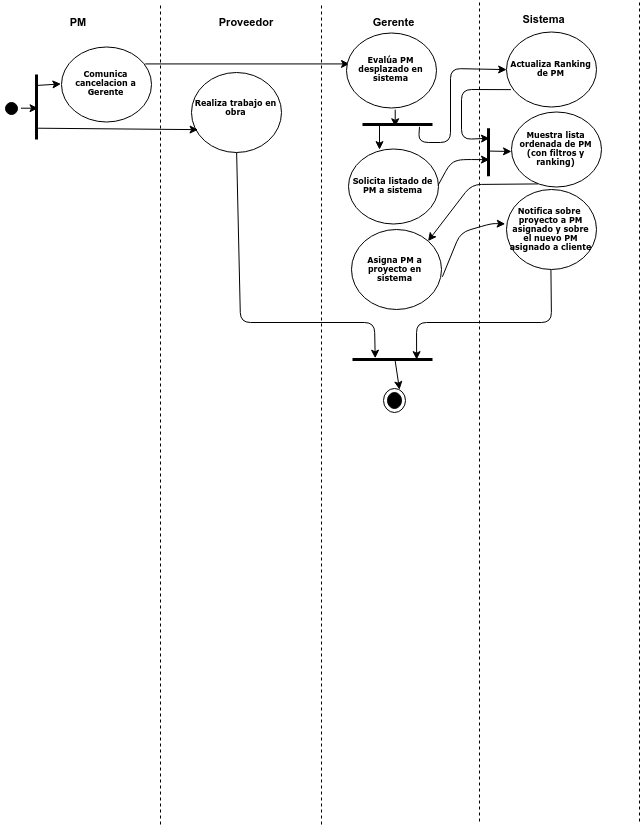
\includegraphics[scale=0.5, angle=90]{imagenes/DA4.png}
\end{center}
